% Options for packages loaded elsewhere
\PassOptionsToPackage{unicode}{hyperref}
\PassOptionsToPackage{hyphens}{url}
%
\documentclass[
  11pt,
]{article}
\usepackage{amsmath,amssymb}
\usepackage{lmodern}
\usepackage{iftex}
\ifPDFTeX
  \usepackage[T1]{fontenc}
  \usepackage[utf8]{inputenc}
  \usepackage{textcomp} % provide euro and other symbols
\else % if luatex or xetex
  \usepackage{unicode-math}
  \defaultfontfeatures{Scale=MatchLowercase}
  \defaultfontfeatures[\rmfamily]{Ligatures=TeX,Scale=1}
\fi
% Use upquote if available, for straight quotes in verbatim environments
\IfFileExists{upquote.sty}{\usepackage{upquote}}{}
\IfFileExists{microtype.sty}{% use microtype if available
  \usepackage[]{microtype}
  \UseMicrotypeSet[protrusion]{basicmath} % disable protrusion for tt fonts
}{}
\makeatletter
\@ifundefined{KOMAClassName}{% if non-KOMA class
  \IfFileExists{parskip.sty}{%
    \usepackage{parskip}
  }{% else
    \setlength{\parindent}{0pt}
    \setlength{\parskip}{6pt plus 2pt minus 1pt}}
}{% if KOMA class
  \KOMAoptions{parskip=half}}
\makeatother
\usepackage{xcolor}
\IfFileExists{xurl.sty}{\usepackage{xurl}}{} % add URL line breaks if available
\IfFileExists{bookmark.sty}{\usepackage{bookmark}}{\usepackage{hyperref}}
\hypersetup{
  pdftitle={SURVIVAL ANALYSIS - TCGA PRAD CANCER},
  pdfauthor={Kelvin Ofori-Minta; University of Texas at El Paso (UTEP)},
  hidelinks,
  pdfcreator={LaTeX via pandoc}}
\urlstyle{same} % disable monospaced font for URLs
\usepackage[margin=1in]{geometry}
\usepackage{color}
\usepackage{fancyvrb}
\newcommand{\VerbBar}{|}
\newcommand{\VERB}{\Verb[commandchars=\\\{\}]}
\DefineVerbatimEnvironment{Highlighting}{Verbatim}{commandchars=\\\{\}}
% Add ',fontsize=\small' for more characters per line
\usepackage{framed}
\definecolor{shadecolor}{RGB}{248,248,248}
\newenvironment{Shaded}{\begin{snugshade}}{\end{snugshade}}
\newcommand{\AlertTok}[1]{\textcolor[rgb]{0.94,0.16,0.16}{#1}}
\newcommand{\AnnotationTok}[1]{\textcolor[rgb]{0.56,0.35,0.01}{\textbf{\textit{#1}}}}
\newcommand{\AttributeTok}[1]{\textcolor[rgb]{0.77,0.63,0.00}{#1}}
\newcommand{\BaseNTok}[1]{\textcolor[rgb]{0.00,0.00,0.81}{#1}}
\newcommand{\BuiltInTok}[1]{#1}
\newcommand{\CharTok}[1]{\textcolor[rgb]{0.31,0.60,0.02}{#1}}
\newcommand{\CommentTok}[1]{\textcolor[rgb]{0.56,0.35,0.01}{\textit{#1}}}
\newcommand{\CommentVarTok}[1]{\textcolor[rgb]{0.56,0.35,0.01}{\textbf{\textit{#1}}}}
\newcommand{\ConstantTok}[1]{\textcolor[rgb]{0.00,0.00,0.00}{#1}}
\newcommand{\ControlFlowTok}[1]{\textcolor[rgb]{0.13,0.29,0.53}{\textbf{#1}}}
\newcommand{\DataTypeTok}[1]{\textcolor[rgb]{0.13,0.29,0.53}{#1}}
\newcommand{\DecValTok}[1]{\textcolor[rgb]{0.00,0.00,0.81}{#1}}
\newcommand{\DocumentationTok}[1]{\textcolor[rgb]{0.56,0.35,0.01}{\textbf{\textit{#1}}}}
\newcommand{\ErrorTok}[1]{\textcolor[rgb]{0.64,0.00,0.00}{\textbf{#1}}}
\newcommand{\ExtensionTok}[1]{#1}
\newcommand{\FloatTok}[1]{\textcolor[rgb]{0.00,0.00,0.81}{#1}}
\newcommand{\FunctionTok}[1]{\textcolor[rgb]{0.00,0.00,0.00}{#1}}
\newcommand{\ImportTok}[1]{#1}
\newcommand{\InformationTok}[1]{\textcolor[rgb]{0.56,0.35,0.01}{\textbf{\textit{#1}}}}
\newcommand{\KeywordTok}[1]{\textcolor[rgb]{0.13,0.29,0.53}{\textbf{#1}}}
\newcommand{\NormalTok}[1]{#1}
\newcommand{\OperatorTok}[1]{\textcolor[rgb]{0.81,0.36,0.00}{\textbf{#1}}}
\newcommand{\OtherTok}[1]{\textcolor[rgb]{0.56,0.35,0.01}{#1}}
\newcommand{\PreprocessorTok}[1]{\textcolor[rgb]{0.56,0.35,0.01}{\textit{#1}}}
\newcommand{\RegionMarkerTok}[1]{#1}
\newcommand{\SpecialCharTok}[1]{\textcolor[rgb]{0.00,0.00,0.00}{#1}}
\newcommand{\SpecialStringTok}[1]{\textcolor[rgb]{0.31,0.60,0.02}{#1}}
\newcommand{\StringTok}[1]{\textcolor[rgb]{0.31,0.60,0.02}{#1}}
\newcommand{\VariableTok}[1]{\textcolor[rgb]{0.00,0.00,0.00}{#1}}
\newcommand{\VerbatimStringTok}[1]{\textcolor[rgb]{0.31,0.60,0.02}{#1}}
\newcommand{\WarningTok}[1]{\textcolor[rgb]{0.56,0.35,0.01}{\textbf{\textit{#1}}}}
\usepackage{graphicx}
\makeatletter
\def\maxwidth{\ifdim\Gin@nat@width>\linewidth\linewidth\else\Gin@nat@width\fi}
\def\maxheight{\ifdim\Gin@nat@height>\textheight\textheight\else\Gin@nat@height\fi}
\makeatother
% Scale images if necessary, so that they will not overflow the page
% margins by default, and it is still possible to overwrite the defaults
% using explicit options in \includegraphics[width, height, ...]{}
\setkeys{Gin}{width=\maxwidth,height=\maxheight,keepaspectratio}
% Set default figure placement to htbp
\makeatletter
\def\fps@figure{htbp}
\makeatother
\setlength{\emergencystretch}{3em} % prevent overfull lines
\providecommand{\tightlist}{%
  \setlength{\itemsep}{0pt}\setlength{\parskip}{0pt}}
\setcounter{secnumdepth}{5}
\usepackage{amsmath}
\usepackage{amssymb, bm}
\usepackage{amsfonts}
\usepackage{amsthm}
\usepackage{fancyhdr}
\pagestyle{fancy}
\fancyhf{}
\rhead{Collaborative Research}
\lhead{Thyroid Cancer}
\cfoot{\thepage}
\usepackage{algorithm}
\usepackage[noend]{algpseudocode}
\usepackage{booktabs}
\usepackage{longtable}
\usepackage{array}
\usepackage{multirow}
\usepackage{wrapfig}
\usepackage{float}
\usepackage{colortbl}
\usepackage{pdflscape}
\usepackage{tabu}
\usepackage{threeparttable}
\usepackage{threeparttablex}
\usepackage[normalem]{ulem}
\usepackage{makecell}
\usepackage{xcolor}
\ifLuaTeX
  \usepackage{selnolig}  % disable illegal ligatures
\fi

\title{SURVIVAL ANALYSIS - TCGA PRAD CANCER}
\author{Kelvin Ofori-Minta \and University of Texas at El Paso (UTEP)}
\date{June 27, 2022}

\begin{document}
\maketitle

{
\setcounter{tocdepth}{4}
\tableofcontents
}
\section{Loading and Cleaning Data}

\begin{Shaded}
\begin{Highlighting}[]
\NormalTok{data }\OtherTok{\textless{}{-}} \FunctionTok{read.csv}\NormalTok{(}\StringTok{"thyroidcancer.csv"}\NormalTok{, }\AttributeTok{header =}\NormalTok{ T, }\AttributeTok{na.strings =} \StringTok{"NA"}\NormalTok{)}

\NormalTok{data[data}\SpecialCharTok{==}\StringTok{""}\NormalTok{]}\OtherTok{\textless{}{-}}\ConstantTok{NA} \CommentTok{\#replace all empty cells with na}

\CommentTok{\# write.csv(data,"C://Users//Kelvin//Desktop//Spring 2022//research with Dr. Leung//survival//selected\_columns.csv")}
\end{Highlighting}
\end{Shaded}

\subsection{Inspecting dataframe for missing values}

\begin{Shaded}
\begin{Highlighting}[]
\FunctionTok{require}\NormalTok{(inspectdf)}
\FunctionTok{show\_plot}\NormalTok{(}\FunctionTok{inspect\_na}\NormalTok{(data))}
\end{Highlighting}
\end{Shaded}

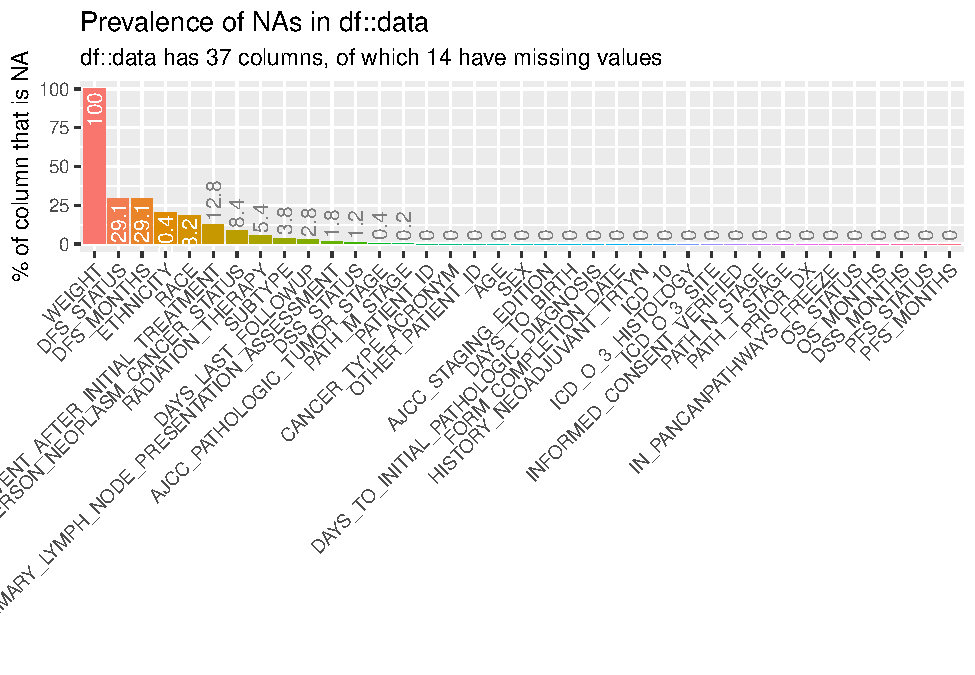
\includegraphics{thyroid_1_files/figure-latex/unnamed-chunk-2-1.pdf}

\begin{Shaded}
\begin{Highlighting}[]
\NormalTok{missing }\OtherTok{=} \FunctionTok{inspect\_na}\NormalTok{(data)}
\NormalTok{missing[ , }\DecValTok{3}\NormalTok{] }\OtherTok{=} \FunctionTok{round}\NormalTok{(missing[ ,}\DecValTok{3}\NormalTok{], }\DecValTok{2}\NormalTok{)}
\FunctionTok{names}\NormalTok{(missing) }\OtherTok{=} \FunctionTok{c}\NormalTok{(}\StringTok{"variable"}\NormalTok{, }\StringTok{"count"}\NormalTok{, }\StringTok{"proportion"}\NormalTok{)}
\FunctionTok{require}\NormalTok{(kableExtra)}
\FunctionTok{kable}\NormalTok{(missing)}
\end{Highlighting}
\end{Shaded}

\begin{tabular}{l|r|r}
\hline
variable & count & proportion\\
\hline
WEIGHT & 499 & 100.00\\
\hline
DFS\_STATUS & 145 & 29.06\\
\hline
DFS\_MONTHS & 145 & 29.06\\
\hline
ETHNICITY & 102 & 20.44\\
\hline
RACE & 91 & 18.24\\
\hline
NEW\_TUMOR\_EVENT\_AFTER\_INITIAL\_TREATMENT & 64 & 12.83\\
\hline
PERSON\_NEOPLASM\_CANCER\_STATUS & 42 & 8.42\\
\hline
RADIATION\_THERAPY & 27 & 5.41\\
\hline
SUBTYPE & 19 & 3.81\\
\hline
DAYS\_LAST\_FOLLOWUP & 14 & 2.81\\
\hline
PRIMARY\_LYMPH\_NODE\_PRESENTATION\_ASSESSMENT & 9 & 1.80\\
\hline
DSS\_STATUS & 6 & 1.20\\
\hline
AJCC\_PATHOLOGIC\_TUMOR\_STAGE & 2 & 0.40\\
\hline
PATH\_M\_STAGE & 1 & 0.20\\
\hline
PATIENT\_ID & 0 & 0.00\\
\hline
CANCER\_TYPE\_ACRONYM & 0 & 0.00\\
\hline
OTHER\_PATIENT\_ID & 0 & 0.00\\
\hline
AGE & 0 & 0.00\\
\hline
SEX & 0 & 0.00\\
\hline
AJCC\_STAGING\_EDITION & 0 & 0.00\\
\hline
DAYS\_TO\_BIRTH & 0 & 0.00\\
\hline
DAYS\_TO\_INITIAL\_PATHOLOGIC\_DIAGNOSIS & 0 & 0.00\\
\hline
FORM\_COMPLETION\_DATE & 0 & 0.00\\
\hline
HISTORY\_NEOADJUVANT\_TRTYN & 0 & 0.00\\
\hline
ICD\_10 & 0 & 0.00\\
\hline
ICD\_O\_3\_HISTOLOGY & 0 & 0.00\\
\hline
ICD\_O\_3\_SITE & 0 & 0.00\\
\hline
INFORMED\_CONSENT\_VERIFIED & 0 & 0.00\\
\hline
PATH\_N\_STAGE & 0 & 0.00\\
\hline
PATH\_T\_STAGE & 0 & 0.00\\
\hline
PRIOR\_DX & 0 & 0.00\\
\hline
IN\_PANCANPATHWAYS\_FREEZE & 0 & 0.00\\
\hline
OS\_STATUS & 0 & 0.00\\
\hline
OS\_MONTHS & 0 & 0.00\\
\hline
DSS\_MONTHS & 0 & 0.00\\
\hline
PFS\_STATUS & 0 & 0.00\\
\hline
PFS\_MONTHS & 0 & 0.00\\
\hline
\end{tabular}

\newpage
\subsubsection{Inspect distribution of variables}

\begin{Shaded}
\begin{Highlighting}[]
\NormalTok{explorecolumns\_thyroid}\OtherTok{=}\FunctionTok{c}\NormalTok{(}\StringTok{"AGE"}\NormalTok{,}\StringTok{"SEX"}\NormalTok{,}\StringTok{"PERSON\_NEOPLASM\_CANCER\_STATUS"}\NormalTok{,}\StringTok{"ETHNICITY"}\NormalTok{, }
                           \StringTok{"RACE"}\NormalTok{,}\StringTok{"RADIATION\_THERAPY"}\NormalTok{, }\StringTok{"PFS\_STATUS"}\NormalTok{) }
\NormalTok{dat}\OtherTok{=}\NormalTok{data[,explorecolumns\_thyroid]}

\FunctionTok{colnames}\NormalTok{(dat)[}\FunctionTok{colnames}\NormalTok{(dat)}\SpecialCharTok{==}\StringTok{"PERSON\_NEOPLASM\_CANCER\_STATUS"}\NormalTok{]}\OtherTok{\textless{}{-}}\StringTok{"neoplasm\_status"}

\NormalTok{dat}\SpecialCharTok{$}\NormalTok{PFS\_STATUS}\OtherTok{\textless{}{-}}\FunctionTok{as.integer}\NormalTok{(}\FunctionTok{ifelse}\NormalTok{(dat}\SpecialCharTok{$}\NormalTok{PFS\_STATUS}\SpecialCharTok{==}\StringTok{"0:CENSORED"}\NormalTok{,}\DecValTok{0}\NormalTok{,}\DecValTok{1}\NormalTok{)) }
\NormalTok{dat}\SpecialCharTok{$}\NormalTok{RADIATION\_THERAPY }\OtherTok{=} \FunctionTok{as.integer}\NormalTok{(}\FunctionTok{ifelse}\NormalTok{(dat}\SpecialCharTok{$}\NormalTok{RADIATION\_THERAPY}\SpecialCharTok{==}\StringTok{"No"}\NormalTok{,}\DecValTok{0}\NormalTok{,}\DecValTok{1}\NormalTok{))}
\NormalTok{dat}\SpecialCharTok{$}\NormalTok{SEX }\OtherTok{=} \FunctionTok{as.integer}\NormalTok{(}\FunctionTok{ifelse}\NormalTok{(dat}\SpecialCharTok{$}\NormalTok{SEX}\SpecialCharTok{==}\StringTok{"Female"}\NormalTok{,}\DecValTok{0}\NormalTok{,}\DecValTok{1}\NormalTok{))}
\NormalTok{dat}\SpecialCharTok{$}\NormalTok{neoplasm\_status}\OtherTok{=}\FunctionTok{as.integer}\NormalTok{(}\FunctionTok{ifelse}\NormalTok{(dat}\SpecialCharTok{$}\NormalTok{neoplasm\_status}\SpecialCharTok{==}\StringTok{"Tumor Free"}\NormalTok{,}\DecValTok{0}\NormalTok{,}\DecValTok{1}\NormalTok{))}

\FunctionTok{suppressPackageStartupMessages}\NormalTok{(}\FunctionTok{library}\NormalTok{(tidyverse))}
\NormalTok{dat}\SpecialCharTok{\%\textgreater{}\%}
  \FunctionTok{pivot\_longer}\NormalTok{(}\AttributeTok{cols=}\FunctionTok{c}\NormalTok{(PFS\_STATUS,RADIATION\_THERAPY,AGE, SEX,neoplasm\_status),}
               \AttributeTok{names\_to =}\StringTok{"key"}\NormalTok{, }\AttributeTok{values\_to =} \StringTok{"value"}\NormalTok{, }\FunctionTok{drop\_na}\NormalTok{(dat)) }\SpecialCharTok{\%\textgreater{}\%}
  \FunctionTok{ggplot}\NormalTok{(}\FunctionTok{aes}\NormalTok{(value)) }\SpecialCharTok{+}
  \FunctionTok{geom\_histogram}\NormalTok{(}\AttributeTok{bins =} \DecValTok{20}\NormalTok{) }\SpecialCharTok{+}
  \FunctionTok{facet\_wrap}\NormalTok{(}\SpecialCharTok{\textasciitilde{}}\NormalTok{key, }\AttributeTok{scales=}\StringTok{\textquotesingle{}free\_x\textquotesingle{}}\NormalTok{)}
\end{Highlighting}
\end{Shaded}

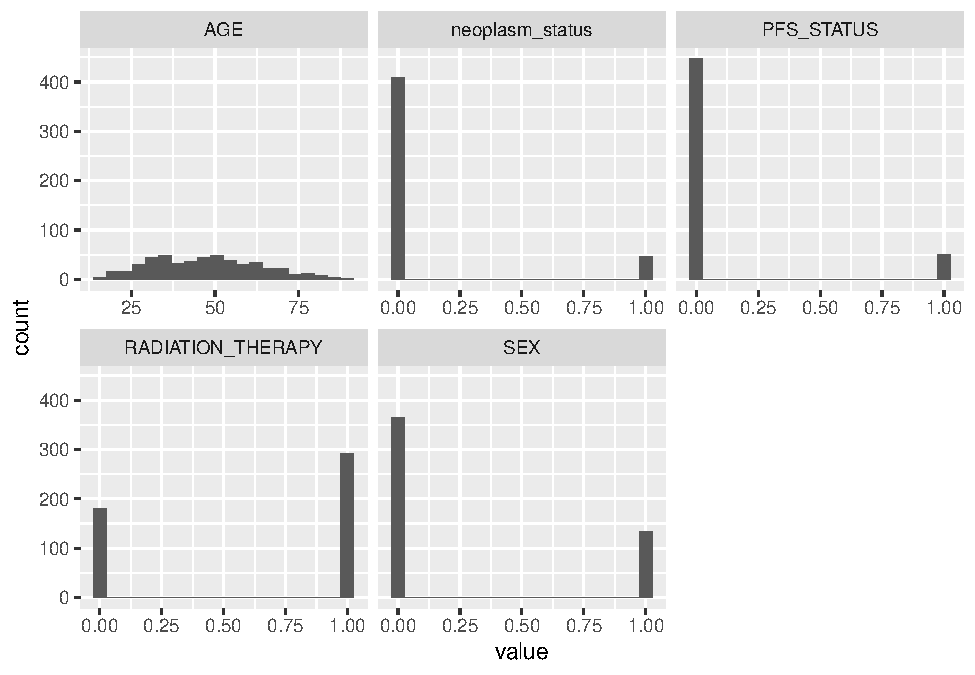
\includegraphics{thyroid_1_files/figure-latex/unnamed-chunk-3-1.pdf}

\newpage
\subsubsection{Re-coding variables}

\begin{Shaded}
\begin{Highlighting}[]
\NormalTok{data}\OtherTok{=}\NormalTok{data[ ,}\SpecialCharTok{{-}}\FunctionTok{c}\NormalTok{(}\DecValTok{28}\NormalTok{)] }\CommentTok{\#remove weight,it has empty cells}


\NormalTok{data}\SpecialCharTok{$}\NormalTok{RADIATION\_THERAPY }\OtherTok{=} \FunctionTok{factor}\NormalTok{(data}\SpecialCharTok{$}\NormalTok{RADIATION\_THERAPY, }\AttributeTok{levels =} \FunctionTok{c}\NormalTok{(}\StringTok{"No"}\NormalTok{,}\StringTok{"Yes"}\NormalTok{),}
                                \AttributeTok{labels =}\FunctionTok{c}\NormalTok{(}\StringTok{"No"}\NormalTok{, }\StringTok{"Yes"}\NormalTok{))}

\NormalTok{data}\SpecialCharTok{$}\NormalTok{SEX }\OtherTok{=} \FunctionTok{factor}\NormalTok{(data}\SpecialCharTok{$}\NormalTok{SEX, }\AttributeTok{levels=}\FunctionTok{c}\NormalTok{(}\StringTok{"Female"}\NormalTok{,}\StringTok{"Male"}\NormalTok{), }\AttributeTok{labels=}\FunctionTok{c}\NormalTok{(}\StringTok{"Female"}\NormalTok{,}\StringTok{"Male"}\NormalTok{))}

\NormalTok{data}\SpecialCharTok{$}\NormalTok{AJCC\_PATHOLOGIC\_TUMOR\_STAGE}\OtherTok{=}\FunctionTok{factor}\NormalTok{(data}\SpecialCharTok{$}\NormalTok{AJCC\_PATHOLOGIC\_TUMOR\_STAGE,}\AttributeTok{levels =} \FunctionTok{c}\NormalTok{(}\StringTok{"STAGE I"}\NormalTok{,}\StringTok{"STAGE II"}\NormalTok{,}\StringTok{"STAGE III"}\NormalTok{,}\StringTok{"STAGE IV"}\NormalTok{,}\StringTok{"STAGE IVA"}\NormalTok{,}\StringTok{"STAGE IVC"}\NormalTok{),}\AttributeTok{labels=}\FunctionTok{c}\NormalTok{(}\StringTok{"STAGE I"}\NormalTok{,}\StringTok{"STAGE II"}\NormalTok{,}\StringTok{"STAGE III"}\NormalTok{,}\StringTok{"STAGE IV"}\NormalTok{,}\StringTok{"STAGE IVA"}\NormalTok{,}\StringTok{"STAGE IVC"}\NormalTok{))}

\NormalTok{data}\SpecialCharTok{$}\NormalTok{AJCC\_STAGING\_EDITION }\OtherTok{=} \FunctionTok{factor}\NormalTok{(data}\SpecialCharTok{$}\NormalTok{AJCC\_STAGING\_EDITION,}
                                   \AttributeTok{levels =} \FunctionTok{c}\NormalTok{(}\StringTok{"4TH"}\NormalTok{,}\StringTok{"5TH"}\NormalTok{,}\StringTok{"6TH"}\NormalTok{,}\StringTok{"7TH"}\NormalTok{),}
                                   \AttributeTok{labels =} \FunctionTok{c}\NormalTok{(}\StringTok{"4TH"}\NormalTok{,}\StringTok{"5TH"}\NormalTok{,}\StringTok{"6TH"}\NormalTok{,}\StringTok{"7TH"}\NormalTok{))}
\NormalTok{data}\SpecialCharTok{$}\NormalTok{ETHNICITY}\OtherTok{=}\FunctionTok{factor}\NormalTok{(data}\SpecialCharTok{$}\NormalTok{ETHNICITY, }
                      \AttributeTok{levels=}\FunctionTok{c}\NormalTok{(}\StringTok{"Hispanic Or Latino"}\NormalTok{, }\StringTok{"Not Hispanic Or Latino"}\NormalTok{),}
                      \AttributeTok{labels =}\FunctionTok{c}\NormalTok{(}\StringTok{"Hispanic Or Latino"}\NormalTok{, }\StringTok{"Not Hispanic Or Latino"}\NormalTok{))}

\NormalTok{data}\SpecialCharTok{$}\NormalTok{PFS\_STATUS}\OtherTok{\textless{}{-}}\FunctionTok{as.integer}\NormalTok{(}\FunctionTok{ifelse}\NormalTok{(data}\SpecialCharTok{$}\NormalTok{PFS\_STATUS}\SpecialCharTok{==}\StringTok{"0:CENSORED"}\NormalTok{,}\DecValTok{0}\NormalTok{,}\DecValTok{1}\NormalTok{)) }
\end{Highlighting}
\end{Shaded}

\newpage
\section{KM Curve - PF Survival of patients with Radiation Therapy}

\begin{Shaded}
\begin{Highlighting}[]
\FunctionTok{library}\NormalTok{(}\StringTok{"survival"}\NormalTok{)}
\FunctionTok{library}\NormalTok{(}\StringTok{"survminer"}\NormalTok{)}
\NormalTok{ndata}\OtherTok{\textless{}{-}}\NormalTok{data}
\NormalTok{fit1}\OtherTok{\textless{}{-}}\FunctionTok{survfit}\NormalTok{(}\FunctionTok{Surv}\NormalTok{(ndata}\SpecialCharTok{$}\NormalTok{PFS\_MONTHS, ndata}\SpecialCharTok{$}\NormalTok{PFS\_STATUS}\SpecialCharTok{==}\DecValTok{1}\NormalTok{)}\SpecialCharTok{\textasciitilde{}}\NormalTok{ndata}\SpecialCharTok{$}\NormalTok{RADIATION\_THERAPY}
\NormalTok{              ,}\AttributeTok{data=}\NormalTok{ndata)}
\FunctionTok{print}\NormalTok{(fit1)}
\end{Highlighting}
\end{Shaded}

\begin{verbatim}
## Call: survfit(formula = Surv(ndata$PFS_MONTHS, ndata$PFS_STATUS == 
##     1) ~ ndata$RADIATION_THERAPY, data = ndata)
## 
##    27 observations deleted due to missingness 
##                               n events median 0.95LCL 0.95UCL
## ndata$RADIATION_THERAPY=No  180     12     NA      NA      NA
## ndata$RADIATION_THERAPY=Yes 292     38     NA      NA      NA
\end{verbatim}

\begin{Shaded}
\begin{Highlighting}[]
\FunctionTok{summary}\NormalTok{(fit1)}\SpecialCharTok{$}\NormalTok{table}
\end{Highlighting}
\end{Shaded}

\begin{verbatim}
##                             records n.max n.start events    rmean se(rmean)
## ndata$RADIATION_THERAPY=No      180   180     180     12 162.8716  4.441883
## ndata$RADIATION_THERAPY=Yes     292   292     292     38 147.8427  4.827914
##                             median 0.95LCL 0.95UCL
## ndata$RADIATION_THERAPY=No      NA      NA      NA
## ndata$RADIATION_THERAPY=Yes     NA      NA      NA
\end{verbatim}

\newpage

\begin{Shaded}
\begin{Highlighting}[]
\FunctionTok{ggsurvplot}\NormalTok{(fit1,}
          \CommentTok{\#legend.labs=c("tumor\_free", "with\_tumor"),}
          \AttributeTok{pval =} \ConstantTok{TRUE}\NormalTok{, }\AttributeTok{conf.int =}\NormalTok{ F,}
          \AttributeTok{risk.table =} \ConstantTok{TRUE}\NormalTok{, }\CommentTok{\# Add risk table}
          \AttributeTok{risk.table.col =} \StringTok{"strata"}\NormalTok{, }\CommentTok{\# Change risk table color by groups}
          \AttributeTok{linetype =} \StringTok{"strata"}\NormalTok{, }\CommentTok{\# Change line type by groups}
          \AttributeTok{surv.median.line =} \StringTok{"hv"}\NormalTok{, }\CommentTok{\# Specify median survival}
          \AttributeTok{ggtheme =} \FunctionTok{theme\_bw}\NormalTok{(), }\CommentTok{\# Change ggplot2 theme}
          \AttributeTok{palette =} \FunctionTok{c}\NormalTok{(}\StringTok{"\#E7B800"}\NormalTok{, }\StringTok{"\#2E9FDF"}\NormalTok{))}
\end{Highlighting}
\end{Shaded}

\begin{verbatim}
## Warning in .add_surv_median(p, fit, type = surv.median.line, fun = fun, : Median
## survival not reached.
\end{verbatim}

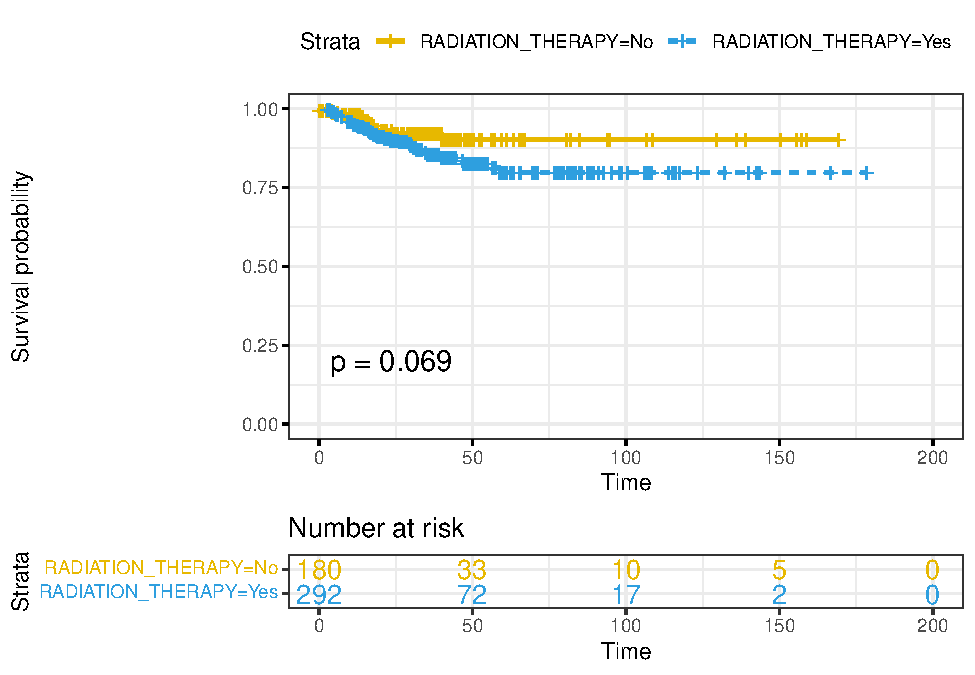
\includegraphics{thyroid_1_files/figure-latex/unnamed-chunk-6-1.pdf}

\newpage
\section{PF Survival of Neoplasm Tumor Patients Exposed to Radiation Therapy}

\begin{Shaded}
\begin{Highlighting}[]
\NormalTok{tumor}\OtherTok{=}\NormalTok{ndata[ndata}\SpecialCharTok{$}\NormalTok{PERSON\_NEOPLASM\_CANCER\_STATUS}\SpecialCharTok{==}\StringTok{"With Tumor"}\NormalTok{,]}

\NormalTok{fit2}\OtherTok{\textless{}{-}}\FunctionTok{survfit}\NormalTok{(}\FunctionTok{Surv}\NormalTok{(tumor}\SpecialCharTok{$}\NormalTok{PFS\_MONTHS, tumor}\SpecialCharTok{$}\NormalTok{PFS\_STATUS}\SpecialCharTok{==}\DecValTok{1}\NormalTok{)}\SpecialCharTok{\textasciitilde{}}\NormalTok{tumor}\SpecialCharTok{$}\NormalTok{RADIATION\_THERAPY}
\NormalTok{              ,}\AttributeTok{data=}\NormalTok{tumor)}

\FunctionTok{print}\NormalTok{(fit2)}
\end{Highlighting}
\end{Shaded}

\begin{verbatim}
## Call: survfit(formula = Surv(tumor$PFS_MONTHS, tumor$PFS_STATUS == 
##     1) ~ tumor$RADIATION_THERAPY, data = tumor)
## 
##    44 observations deleted due to missingness 
##                              n events median 0.95LCL 0.95UCL
## tumor$RADIATION_THERAPY=No   5      4   15.9    14.2      NA
## tumor$RADIATION_THERAPY=Yes 40     17   45.5    29.7      NA
\end{verbatim}

\begin{Shaded}
\begin{Highlighting}[]
\FunctionTok{summary}\NormalTok{(fit2)}\SpecialCharTok{$}\NormalTok{table}
\end{Highlighting}
\end{Shaded}

\begin{verbatim}
##                             records n.max n.start events    rmean se(rmean)
## tumor$RADIATION_THERAPY=No        5     5       5      4 13.61739  2.224726
## tumor$RADIATION_THERAPY=Yes      40    40      40     17 62.56331 13.398065
##                               median  0.95LCL 0.95UCL
## tumor$RADIATION_THERAPY=No  15.87928 14.16971      NA
## tumor$RADIATION_THERAPY=Yes 45.53375 29.68735      NA
\end{verbatim}

\begin{Shaded}
\begin{Highlighting}[]
\FunctionTok{ggsurvplot}\NormalTok{(fit2,}
          \AttributeTok{pval =} \ConstantTok{TRUE}\NormalTok{, }\AttributeTok{conf.int =}\NormalTok{ F,}
          \AttributeTok{risk.table =} \ConstantTok{TRUE}\NormalTok{, }\CommentTok{\# Add risk table}
          \AttributeTok{risk.table.col =} \StringTok{"strata"}\NormalTok{, }\CommentTok{\# Change risk table color by groups}
          \AttributeTok{linetype =} \StringTok{"strata"}\NormalTok{, }\CommentTok{\# Change line type by groups}
          \AttributeTok{surv.median.line =} \StringTok{"hv"}\NormalTok{, }\CommentTok{\# Specify median survival}
          \AttributeTok{ggtheme =} \FunctionTok{theme\_bw}\NormalTok{(), }\CommentTok{\# Change ggplot2 theme}
          \AttributeTok{palette =} \FunctionTok{c}\NormalTok{(}\StringTok{"\#E7B800"}\NormalTok{, }\StringTok{"\#2E9FDF"}\NormalTok{))}
\end{Highlighting}
\end{Shaded}

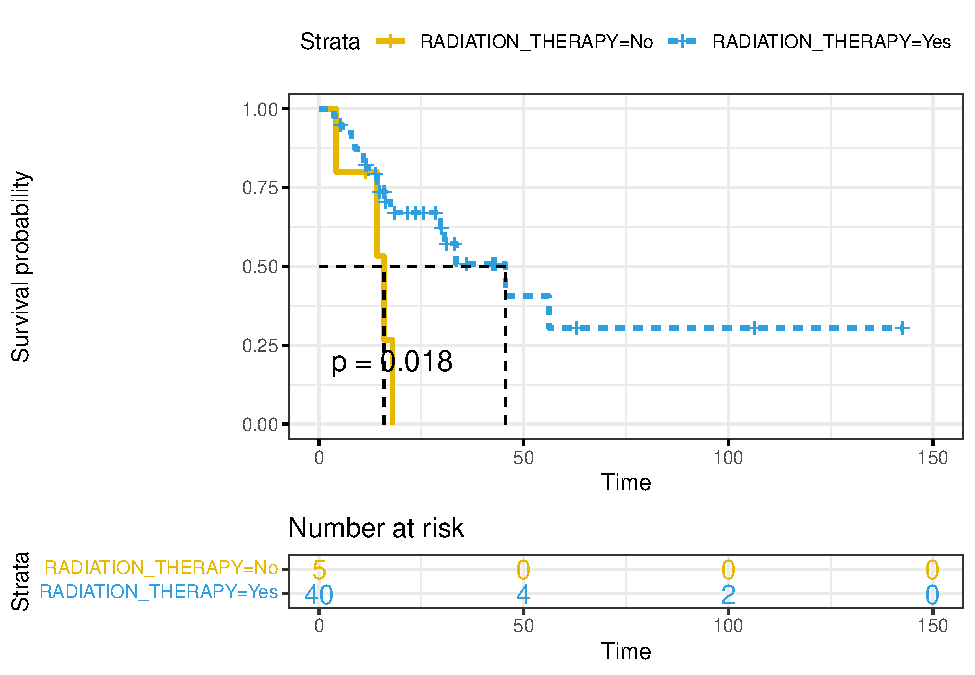
\includegraphics{thyroid_1_files/figure-latex/unnamed-chunk-8-1.pdf}

\begin{Shaded}
\begin{Highlighting}[]
\FunctionTok{table}\NormalTok{(data}\SpecialCharTok{$}\NormalTok{PERSON\_NEOPLASM\_CANCER\_STATUS)}
\end{Highlighting}
\end{Shaded}

\begin{verbatim}
## 
## Tumor Free With Tumor 
##        410         47
\end{verbatim}

\begin{Shaded}
\begin{Highlighting}[]
\FunctionTok{table}\NormalTok{(tumor}\SpecialCharTok{$}\NormalTok{PFS\_STATUS)}
\end{Highlighting}
\end{Shaded}

\begin{verbatim}
## 
##  0  1 
## 25 22
\end{verbatim}

\begin{Shaded}
\begin{Highlighting}[]
\FunctionTok{table}\NormalTok{(tumor}\SpecialCharTok{$}\NormalTok{RADIATION\_THERAPY)}
\end{Highlighting}
\end{Shaded}

\begin{verbatim}
## 
##  No Yes 
##   5  40
\end{verbatim}

\newpage
\section{Logrank Test}

\begin{Shaded}
\begin{Highlighting}[]
\NormalTok{logrank }\OtherTok{\textless{}{-}} \FunctionTok{survdiff}\NormalTok{(}\FunctionTok{Surv}\NormalTok{(tumor}\SpecialCharTok{$}\NormalTok{PFS\_MONTHS, tumor}\SpecialCharTok{$}\NormalTok{PFS\_STATUS}\SpecialCharTok{==}\DecValTok{1}\NormalTok{)}\SpecialCharTok{\textasciitilde{}}\NormalTok{tumor}\SpecialCharTok{$}\NormalTok{RADIATION\_THERAPY}
\NormalTok{              ,}\AttributeTok{data=}\NormalTok{tumor)}
\NormalTok{logrank}
\end{Highlighting}
\end{Shaded}

\begin{verbatim}
## Call:
## survdiff(formula = Surv(tumor$PFS_MONTHS, tumor$PFS_STATUS == 
##     1) ~ tumor$RADIATION_THERAPY, data = tumor)
## 
## n=45, 44 observations deleted due to missingness.
## 
##                              N Observed Expected (O-E)^2/E (O-E)^2/V
## tumor$RADIATION_THERAPY=No   5        4     1.37     5.077      5.59
## tumor$RADIATION_THERAPY=Yes 40       17    19.63     0.353      5.59
## 
##  Chisq= 5.6  on 1 degrees of freedom, p= 0.02
\end{verbatim}

\newpage
\section{Cox Proportional Hazard Model with Neoplasm Tumor Data}

\begin{Shaded}
\begin{Highlighting}[]
\NormalTok{fitph}\OtherTok{\textless{}{-}}\FunctionTok{coxph}\NormalTok{(}\FunctionTok{Surv}\NormalTok{(PFS\_MONTHS,PFS\_STATUS}\SpecialCharTok{==}\DecValTok{1}\NormalTok{) }\SpecialCharTok{\textasciitilde{}}\NormalTok{ RADIATION\_THERAPY }\SpecialCharTok{+}
\NormalTok{                AGE }\SpecialCharTok{+}\NormalTok{ SEX }\SpecialCharTok{+}\NormalTok{ RACE }\SpecialCharTok{+}\NormalTok{ AJCC\_PATHOLOGIC\_TUMOR\_STAGE }\SpecialCharTok{+}\NormalTok{ DAYS\_TO\_BIRTH}
                \SpecialCharTok{+}\NormalTok{ DAYS\_LAST\_FOLLOWUP }\SpecialCharTok{+}\NormalTok{ AJCC\_PATHOLOGIC\_TUMOR\_STAGE }\SpecialCharTok{+}
\NormalTok{               AJCC\_STAGING\_EDITION, }
             \AttributeTok{data=}\NormalTok{tumor)}
\FunctionTok{summary}\NormalTok{(fitph)}
\end{Highlighting}
\end{Shaded}

\begin{verbatim}
## Call:
## coxph(formula = Surv(PFS_MONTHS, PFS_STATUS == 1) ~ RADIATION_THERAPY + 
##     AGE + SEX + RACE + AJCC_PATHOLOGIC_TUMOR_STAGE + DAYS_TO_BIRTH + 
##     DAYS_LAST_FOLLOWUP + AJCC_PATHOLOGIC_TUMOR_STAGE + AJCC_STAGING_EDITION, 
##     data = tumor)
## 
##   n= 33, number of events= 15 
##    (56 observations deleted due to missingness)
## 
##                                            coef  exp(coef)   se(coef)        z
## RADIATION_THERAPYYes                 -1.904e+00  1.489e-01  6.160e-01   -3.091
## AGE                                  -2.226e+00  1.079e-01  1.630e-02 -136.602
## SEXMale                               1.892e+00  6.635e+00  6.387e-01    2.963
## RACEAsian                            -3.683e+01  1.010e-16  4.512e+03   -0.008
## RACEBlack or African American        -1.854e+01  8.897e-09  7.510e-01  -24.684
## RACEWhite                            -1.957e+01  3.158e-09  6.828e-01  -28.665
## AJCC_PATHOLOGIC_TUMOR_STAGESTAGE II   1.751e+01  4.021e+07  1.056e+00   16.579
## AJCC_PATHOLOGIC_TUMOR_STAGESTAGE III  1.698e+01  2.376e+07  5.365e-01   31.658
## AJCC_PATHOLOGIC_TUMOR_STAGESTAGE IV   0.000e+00  1.000e+00  0.000e+00       NA
## AJCC_PATHOLOGIC_TUMOR_STAGESTAGE IVA  1.533e+01  4.537e+06  1.044e+00   14.684
## AJCC_PATHOLOGIC_TUMOR_STAGESTAGE IVC  1.861e+01  1.211e+08  1.234e+00   15.089
## DAYS_TO_BIRTH                        -6.267e-03  9.938e-01  4.470e-05 -140.224
## DAYS_LAST_FOLLOWUP                   -5.606e-04  9.994e-01  2.623e-04   -2.137
## AJCC_STAGING_EDITION5TH              -1.144e+00  3.184e-01  8.234e-01   -1.390
## AJCC_STAGING_EDITION6TH               1.915e+01  2.082e+08  6.831e-01   28.041
## AJCC_STAGING_EDITION7TH               0.000e+00  1.000e+00  6.110e-01    0.000
##                                      Pr(>|z|)    
## RADIATION_THERAPYYes                  0.00199 ** 
## AGE                                   < 2e-16 ***
## SEXMale                               0.00305 ** 
## RACEAsian                             0.99349    
## RACEBlack or African American         < 2e-16 ***
## RACEWhite                             < 2e-16 ***
## AJCC_PATHOLOGIC_TUMOR_STAGESTAGE II   < 2e-16 ***
## AJCC_PATHOLOGIC_TUMOR_STAGESTAGE III  < 2e-16 ***
## AJCC_PATHOLOGIC_TUMOR_STAGESTAGE IV        NA    
## AJCC_PATHOLOGIC_TUMOR_STAGESTAGE IVA  < 2e-16 ***
## AJCC_PATHOLOGIC_TUMOR_STAGESTAGE IVC  < 2e-16 ***
## DAYS_TO_BIRTH                         < 2e-16 ***
## DAYS_LAST_FOLLOWUP                    0.03257 *  
## AJCC_STAGING_EDITION5TH               0.16459    
## AJCC_STAGING_EDITION6TH               < 2e-16 ***
## AJCC_STAGING_EDITION7TH               1.00000    
## ---
## Signif. codes:  0 '***' 0.001 '**' 0.01 '*' 0.05 '.' 0.1 ' ' 1
## 
##                                      exp(coef) exp(-coef) lower .95 upper .95
## RADIATION_THERAPYYes                 1.489e-01  6.714e+00 4.453e-02 4.981e-01
## AGE                                  1.079e-01  9.267e+00 1.045e-01 1.114e-01
## SEXMale                              6.635e+00  1.507e-01 1.897e+00 2.320e+01
## RACEAsian                            1.010e-16  9.906e+15 0.000e+00       Inf
## RACEBlack or African American        8.897e-09  1.124e+08 2.042e-09 3.877e-08
## RACEWhite                            3.158e-09  3.166e+08 8.284e-10 1.204e-08
## AJCC_PATHOLOGIC_TUMOR_STAGESTAGE II  4.021e+07  2.487e-08 5.074e+06 3.187e+08
## AJCC_PATHOLOGIC_TUMOR_STAGESTAGE III 2.376e+07  4.210e-08 8.301e+06 6.798e+07
## AJCC_PATHOLOGIC_TUMOR_STAGESTAGE IV  1.000e+00  1.000e+00 1.000e+00 1.000e+00
## AJCC_PATHOLOGIC_TUMOR_STAGESTAGE IVA 4.537e+06  2.204e-07 5.865e+05 3.510e+07
## AJCC_PATHOLOGIC_TUMOR_STAGESTAGE IVC 1.211e+08  8.256e-09 1.079e+07 1.359e+09
## DAYS_TO_BIRTH                        9.938e-01  1.006e+00 9.937e-01 9.938e-01
## DAYS_LAST_FOLLOWUP                   9.994e-01  1.001e+00 9.989e-01 1.000e+00
## AJCC_STAGING_EDITION5TH              3.184e-01  3.140e+00 6.341e-02 1.599e+00
## AJCC_STAGING_EDITION6TH              2.082e+08  4.803e-09 5.458e+07 7.941e+08
## AJCC_STAGING_EDITION7TH              1.000e+00  1.000e+00 3.020e-01 3.312e+00
## 
## Concordance= 0.869  (se = 0.049 )
## Likelihood ratio test= 30.75  on 16 df,   p=0.01
## Wald test            = 22618  on 16 df,   p=<2e-16
## Score (logrank) test = 32.25  on 16 df,   p=0.009
\end{verbatim}

\newpage
\section{}

\end{document}
